\documentclass{standalone}
\usepackage{tikz}
\usetikzlibrary{arrows.meta} % For better arrowheads

\begin{document}

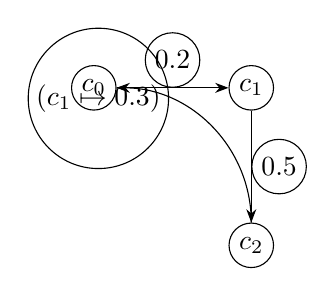
\begin{tikzpicture}[>=Stealth, % Set arrow style
    every node/.style={circle, draw, inner sep=2pt}, % Style for nodes
    label distance=3mm % Distance between node and label
]

% Define nodes
\node (c0) at (0,0) {$c_0$};
\node (c1) at (2,0) {$c_1$};
\node (c2) at (2,-2) {$c_2$};

% Draw edges with labels
\draw[->] (c0) -- node[above] {0.2} (c1); % Edge from c0 to c1
\draw[->] (c1) -- node[right] {0.5} (c2); % Edge from c1 to c2
\draw[->, bend right=45] (c2) to node[left, pos=0.75] {$(c_1 \mapsto 0.3)$} (c0); % Curved edge from c2 to c0

\end{tikzpicture}

\end{document}